% !TEX encoding = UTF-8
% !TEX TS-program = pdflatex
% !TEX root = ../relazione-finale.tex

%**************************************************************
\chapter{Introduzione}
\label{cap:introduzione}
%**************************************************************

% \noindent Esempio di utilizzo di un termine nel glossario \\
% \gls{api}. \\
%
% \noindent Esempio di citazione in linea \\
% \cite{site:agile-manifesto}. \\
%
% \noindent Esempio di citazione nel pie' di pagina \\
% citazione\footcite{womak:lean-thinking} \\

%**************************************************************
\section{L'idea}

% obiettivi dello stage

% caratteristiche dello stage

In questa relazione descrivo lo svolgimento dello stage effettuato nel contesto del Corso di Laurea di Informatica dell'Università di Padova.

Ho intrapreso lo stage nella sua forma interna individuale, in cui con il proponente, \profTitle \myProf, ho redatto un piano di lavoro nel quale lo stage abbia una durata pianificata su 300 ore.

L'obiettivo principale dello stage consiste nello sviluppo e nella realizzazione di un prototipo per la gestione di dispositivi interconnessi (IoT) attraverso un'interfaccia \emph{web}.
Questo centro di controllo attraverso cui l'utente del sistema gestisce i dispositivi \emph{smart} presenti nella propria rete domestica dovrebbe permettere operazioni quali:
\begin{itemize}
  \item avvio/spegnimento di un dispositivo;
  \item monitoraggio dei dispositivi collegati;
  \item collegamento all'eventuale interfaccia proprietaria del dispositivo (es. supporto tecnico).
\end{itemize}

Ho sviluppato e realizzato il progetto di stage con l'idea di unificare in un unico centro di controllo tutti gli eventuali dispositivi connessi alla rete domestica dell'utente, permettendo tuttavia allo stesso di accedere all'interfaccia proprietaria di ciascun dispositivo.
L'obiettivo di una tale \emph{dashboard} non è quindi confinare l'utente in un unico ecosistema domotico,
bensì quello di facilitare la consultazione delle informazioni più frequentemente richieste dall'utente provenienti da più ecosistemi distinti. \\
Grazie alla natura prototipale del prodotto sviluppato, ho inoltre potuto sperimentare l'approccio architetturale a microservizi, al fine di garantire scalabilità all'applicazione.

%**************************************************************
\section{IoT: definizione e caratteristiche generali}
\label{intro-iot}

\emph{Internet Of Things} è un paradigma tecnologico diffusosi nell'ultimo decennio. Questa locuzione fa riferimento a un insieme di oggetti,
di varia natura e utilizzo, che interagiscono tra loro e che permettono all'utente di interagire con essi. \\ \\

Un dispositivo \emph{smart} è un dispositivo elettronico, generalmente connesso ad altri dispositivi, che può svolgere le proprie funzioni in maniera autonoma.
Un esempio lampante di dispositivi \emph{smart} sono gli smartphone, prodotti che hanno arricchito di funzionalità avanzate, interagendo con l'utente in modi precedentemente non possibili, i predecessori telefoni (\emph{phone}).
\footcite{site:smart-device}

Studenti e professori del Dipartimento di Informatica dell'Università di Carnegie Mellon presero in considerazione l'idea di una rete di dispositivi \emph{smart} quando modificarono un distributore automatico di bibite del Dipartimento per accedere al suo inventario di bibite. Quel distributore automatico divenne il primo apparecchio collegato ad Internet.
\footcite{site:mellon-uni}

Nel corso degli anni '90 il mondo accademico e il mondo dell'industra legata alla produzione continuarono a sperimentare evolvendo il \textit{concept} iniziale, arrivando alla conclusione che l'\textit{Ubiquitous Computing} non si debba riferire solamente ai \textit{computer}, ma debba espandersi agli oggetti di utilizzo quotidiano. Questa visione dovette scontrarsi con i limiti della microelettronica di allora: la produzione di semiconduttori non era ancora pronta a supportare la potenziale domanda e i costi per sostenere l'ampliamento degli impianti non erano facilmente assorbibili in breve tempo.
\footcite{site:mit-weiser}

Kevin Ashton coniò il termine \textit{"Internet of Things"} nel 1999.
\footcite{site:iot-kashton}
L'origine dell'espressione, riassumendo le parole dell'autore, deriva dal fatto che la maggior parte delle informazioni presenti su Internet sono state e sono inserite da utenti "umani", soggetti quindi a concentrazione, precisione e tempo limitate;
se queste informazioni fossero invece inserite da macchine senza l'aiuto di un utente umano, la maggior qualità delle stesse garantirebbe:
\setlist{nolistsep}
\begin{itemize}
  \item maggiore capacità di tracciamento delle risorse;
  \item minor spreco di risorse;
  \item minor costo per la gestione delle risorse.
\end{itemize}

Grazie agli avanzamenti nei processi di produzione dei semiconduttori, dovuti alla crescita dei mercati del consumo di massa, allo sviluppo di un numero sempre maggiore di tecnologie volte a migliorare l'efficienza e l'affidabilità dei circuiti integrati e alla sempre maggior diffusione di tecnologie per la trasmissione di informazioni senza fili, dai primi anni 2000 un numero sempre maggiore di aziende, provenienti dagli ambiti più disparati, ha sviluppato il concetto alla base dell'IoT, estendendolo a settori quali \textit{home automation}, \textit{manufacturing}, \textit{smart agriculture}, etc..
\footcite{site:pc-to-things}

\begin{figure}[H]
    \centering
    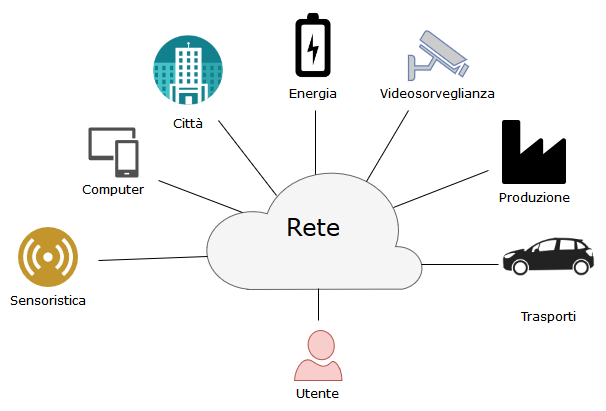
\includegraphics[width=0.9\columnwidth]{intro/iot}
    \caption{Rappresentazione figurata del concetto di \textit{"internet of things"}.}
    \label{fig:iot}
\end{figure}

Posso sintetizzare il concetto di \emph{Internet of Things} come quello di una rete di dispositivi interconnessi, individuabili in modo univoco e che possono comunicare informazioni.
I dispositivi presenti in una rete possono comunicare con due tipologie di attori diverse:
\setlist{nolistsep}
\begin{itemize}
  \item se la comunicazione avviene con altri dispositivi si parla di comunicazione M2M (\textit{Machine to Machine}, ovvero comunicazione tra macchine);
  \item se la comunicazione avviene interagendo con il mondo reale si parla di comunicazione M2H (\textit{Machine to Human}, ovvero comunicazione tra macchina e utente).
\end{itemize}

Il termine "Things" nel contesto IoT si riferisce a una varietà di dispositivi come ad esempio: videocamere di sorveglianza, automobili a guida autonoma e assistita oppure piccoli e grandi elettrodomestici casalinghi. Questi dispositivi, soprannominati anche \textit{smart object}, raccolgono informazioni utili in base agli attori con cui comunicano:
\setlist{nolistsep}
\begin{itemize}
  \item se i dispositivi comunicano in modo M2M, le informazioni supportano tecnologie esistenti, integrandosi nel flusso di informazioni esistente;
  \item se i dispositivi comunicano in modo M2H, le informazioni aiutano le persone che interagiscono con essi.
\end{itemize}

L'interesse verso il tema IoT è cresciuto esponenzialmente sia nel mercato consumer che in quello enterprise e secondo Forbes (\footcite{site:forbes-iot}) diventerà nel prossimo quinquennio uno dei settori dell'ITC più redditizi.
É interessante osservare anche la popolarità dei termini di ricerca correlati all'IoT: i dati sono stati ottenuti interrogando il servizio \url{https://trends.google.com/trends}, il quale consente di effettuare analisi sulla popolarità delle stringhe di ricerca immesse nel motore di ricerca di Google.
Ciascun grafico a linea (\textit{line chart} in inglese) presenta nelle ordinate il grado di popolarità della \textit{query} di ricerca, valutato da 0 (popolarità minima) a 100 (popolarità massima), e nelle ascisse l'arco temporale in analisi.

\begin{figure}[H]
    \centering
    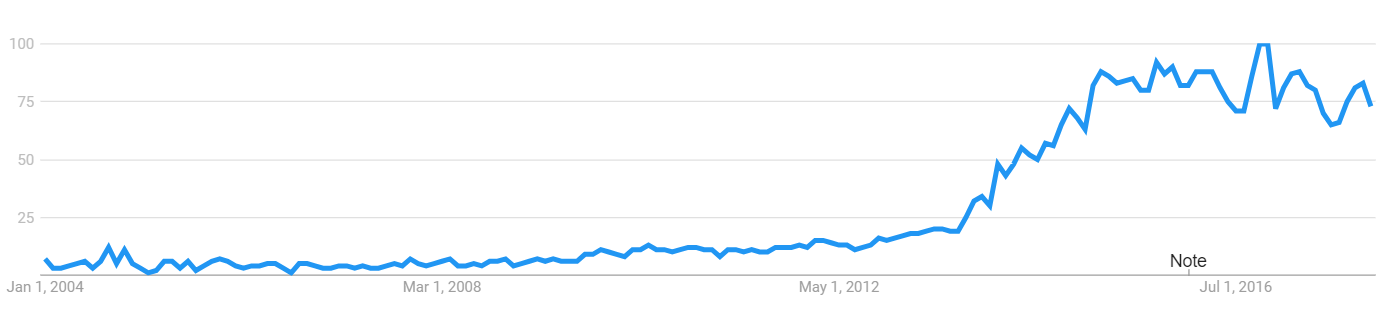
\includegraphics[width=0.9\columnwidth]{intro/internet-of-things-query-interest-worldwide}
    \caption{Andamento dell'interesse per la stringa di ricerca \textit{"internet of things"}. \\ \cite{site:iot-long-trend}}
    \label{fig:internet-of-things-query-interest}
\end{figure}

\begin{figure}[H]
    \centering
    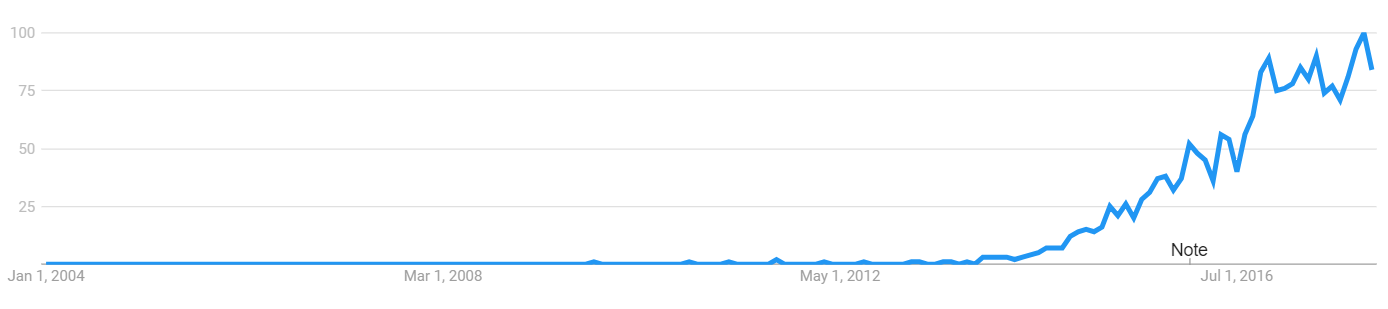
\includegraphics[width=0.9\columnwidth]{intro/iot-devices-query-interest-worldwide}
    \caption{Andamento dell'interesse per la stringa di ricerca \textit{"iot devices"}. \\ \cite{site:iot-devices-trend}}
    \label{fig:iot-devices-query-interest}
\end{figure}

\begin{figure}[H]
    \centering
    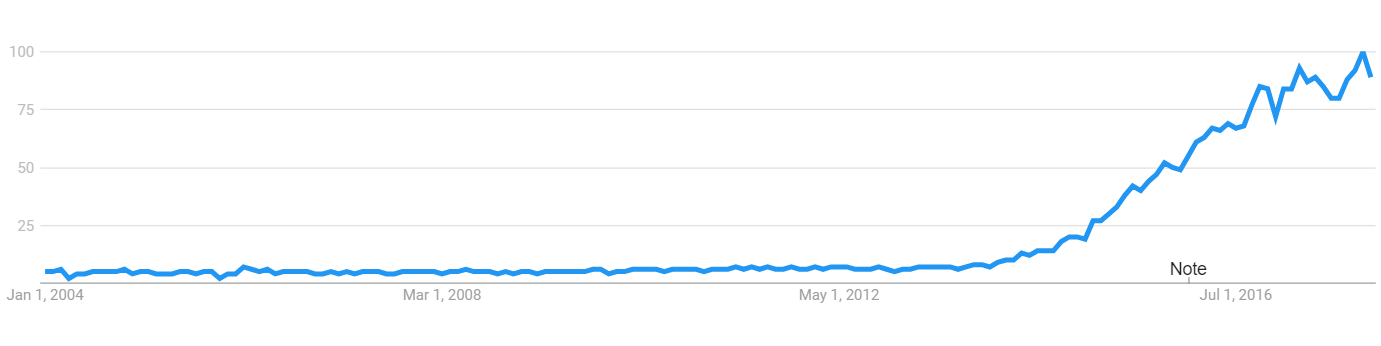
\includegraphics[width=0.9\columnwidth]{intro/iot-query-interest-worldwide}
    \caption{Andamento dell'interesse per la stringa di ricerca \textit{"iot"}. \\ \cite{site:iot-short-trend}}
    \label{fig:iot-query-interest}
\end{figure}

Sintetizzando le previsioni di Forbes con l'andamento dei termini di ricerca legati all'IoT, visibili alle figure ~\ref{fig:internet-of-things-query-interest}, ~\ref{fig:iot-devices-query-interest} e ~\ref{fig:iot-query-interest}, posso evidenziare che l'interesse verso l'argomento IoT stia generalmente aumentando o nel caso peggiore rimanga stabile con l'interesse degli anni precedenti.

\section{Architettura a microservizi: definizione e caratteristiche}
\label{intro:arch}

L'espressione \textbf{Architettura a microservizi} è sempre più comune tra gli sviluppatori di applicazioni \textit{enterprise} per descrivere un metodo di progettazione delle applicazioni come insiemi di servizi eseguibili indipendentemente, che comunicano tra loro grazie a meccanismi di comunicazione "leggeri" (solitamente attraverso \gls{api} HTTP).
Nella concezione originale in cui l'architettura a microservizi è nata, ogni servizio doveva essere progettato per eseguire in un processo indipendente dagli altri; con la nascita e la diffusione dei \emph{container} questo paradigma sta cambiando, associando sempre più l'esecuzione dei microservizi in altrettanti \emph{container}.
La \emph{containerization} (containerizzazione) è un metodo di virtualizzazione posto al livello del sistema operativo per la distribuzione ed esecuzione di applicazioni all'interno di \emph{container}.
\footcite{site:containerization}
Un \emph{container} è un unità \emph{software} standardizzata, distribuibile in un unico pacchetto composto da:
\setlist{nolistsep}
\begin{itemize}
  \itemsep0em
  \item l'applicazione da eseguire;
  \item l'ambiente d'esecuzione configurato correttamente per l'applicazione da eseguire, che a sua volta specifica:
  \begin{itemize}
    \item le dipendenze dell'applicazione;
    \item i file di configurazione dell'applicazione.
  \end{itemize}
\end{itemize}
Una delle tecnologie di containerizzazione che si è più diffusa è \href{https://www.docker.com/what-docker}{Docker} (\url{https://www.docker.com/what-docker}), sviluppata dall'omonima azienda; Docker ha reso disponibile la propria tecnologia di containerizzazione su molteplici piattaforme, sia locali (\emph{computer} con i sistemi operativi \emph{Windows}, \emph{macOS} e i sistemi operativi basati su \emph{Linux}) sia in \emph{cloud} (con ad es. servizi come \emph{Amazon Web Services} e \emph{Microsoft Azure}).
Per implementare il concetto di \emph{container}, la piattaforma di Docker installa un insieme di servizi che comunicano con il \gls{kernelg} del sistema operativo su cui è in esecuzione (\emph{host}) e con i quali gli utenti interagiscono per creare e gestire \emph{container}.
\footcite{site:docker-container}
Ho illustrato l'architettura sopra citata in figura ~\ref{fig:docker-arch}.

\begin{figure}[H]
    \centering
    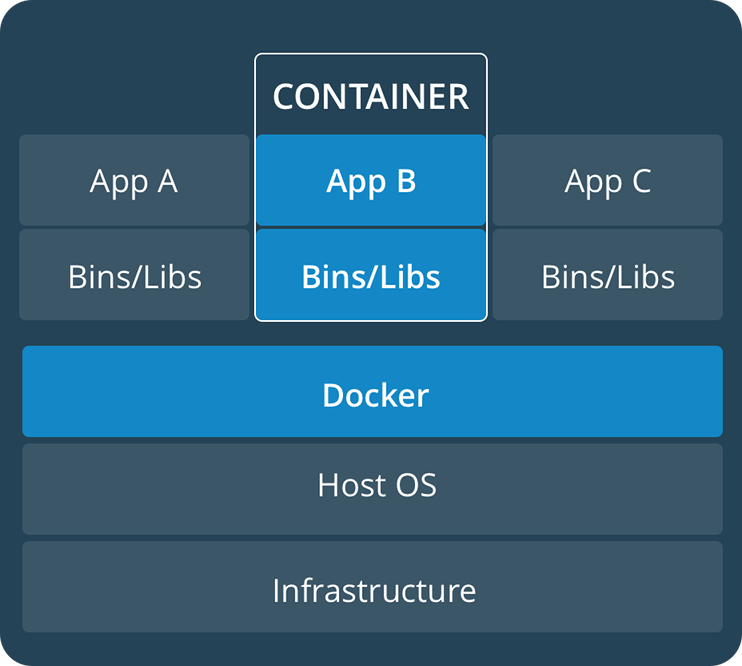
\includegraphics[scale=0.3]{intro/container}
    \caption{Architettura sviluppata da Docker per la sua piattaforma di containerizzazione.\\ \cite{site:docker-container}}
    \label{fig:docker-arch}
\end{figure}

\paragraph{Caratteristiche delle architetture monolitiche}

Un'applicazione monolitica è progettata e costruita per essere una singola unità in esecuzione.
L'applicazione sviluppata con architettura monolitica è responsabile della visualizzazione delle informazioni in un'interfaccia utente (pagine web o \emph{software} nativi), del reperimento delle informazioni da una sorgente di dati (solitamente un \emph{database}) e dell'esecuzione delle logiche di business della stessa.
\footcite{book:beginning-sw-eng}

Nelle applicazioni monolitiche la modularità del sistema si ottiene sfruttando i costrutti fondamentali dell'orientamento ad oggetti presente nei linguaggi di programmazione:
\setlist{nolistsep}
\begin{itemize}
  \item funzioni;
  \item classi;
  \item \emph{namespace} o \emph{package}.
\end{itemize}

\begin{figure}[H]
    \centering
    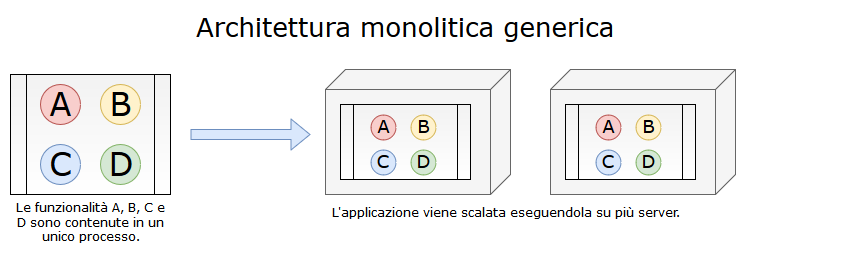
\includegraphics[scale=0.5]{intro/monolith-arch}
    \caption{Caratteristiche di una generica architettura monolitica.\\ \cite{site:fowler-microservices}}
    \label{fig:monolith-arch}
\end{figure}

Per aumentare la disponibilità delle applicazioni monolitiche si usa replicare istanze dell'applicazione in molteplici server, bilanciando il traffico verso le applicazioni per mezzo di un \gls{load balancerg}.
Tra i difetti delle applicazioni monolitiche posso evidenziare:
\setlist{nolistsep}
\begin{itemize}
  \item modifiche a una piccola parte all'applicazione richiedono la ricompilazione e la ridistribuzione dell'applicazione;
  \item all'accrescere della complessità dell'applicazione aumenta anche la difficoltà nel mantenere le modifiche isolate ai moduli di competenza;
  \item scalare l'applicazione richiede l'esecuzione di istanze multiple della stessa applicazione, ignorando di fatto eventuali requisiti di efficienza (solitamente alcune componenti del sistema non richiedono un aumento di \gls{throughputg}).
\end{itemize}

\paragraph{Caratteristiche delle architetture a microservizi}
\label{par:microservizi-intro}

Per lo stile architetturale a microservizi non esistono definizioni formali, tuttavia gli informatici più esperti in materia, tra i quali annovero Martin Fowler, hanno dedotto le caratteristiche che hanno accomunato i progetti diventati nel tempo esempi di best-practice.
Non tutte le architetture a microservizi hanno tutte le caratteristiche elencate in seguito, ma ci si aspetta che la maggior parte delle architetture esibisca quante più caratteristiche possibili.
\footcite{site:fowler-microservices}

L'aspetto cruciale delle architetture a microservizi verte sulla definizione di componente: la definizione comunemente accettata di componente è quella di "unità di software che è indipendentemente aggiornabile e sostituibile in un sistema".
Le architetture a microservizi usano i servizi per realizzare tale definizione di componente. A titolo di confronto con gli approcci di sviluppo tradizionali introduco la nozione di libreria.
Le librerie sono componenti insiti in un'applicazione tanto da risiedere nello stesso spazio di memoria dell'applicazione e che per essere invocate richiedono una chiamata di funzione in memoria.
I servizi sono componenti che vivono nel sistema come processi separati, sfruttando vari tipi di comunicazione interprocesso: richieste web, chiamate di funzione remote (RPC).
\footcite{site:fowler-microservices}

Il vantaggio principale dei servizi rispetto alle librerie consiste nel fatto che i servizi sono rilasciabili indipendentemente dal sistema.
Data la natura dell'architettura a microservizi, modifiche a un singolo servizio comportano il rilascio di una nuova versione solamente per quel servizio e non dell'intera applicazione.
Una buona architettura a microservizi quindi mira a progettare e implementare servizi che circoscrivano chiaramente il loro scopo.

\begin{figure}[H]
    \centering
    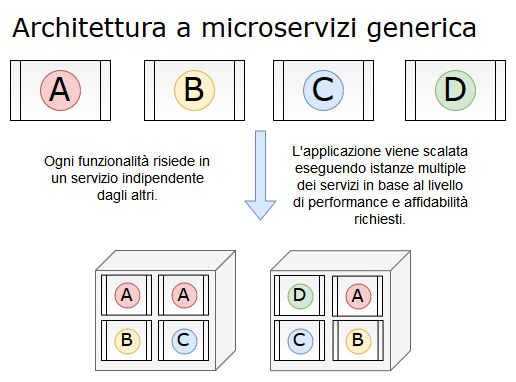
\includegraphics[scale=0.5]{intro/microservices-arch}
    \caption{Caratteristiche di una generica architettura a microservizi.\\ \cite{site:fowler-microservices}}
    \label{fig:microservices-arch}
\end{figure}

L'uso di servizi come componenti consente inoltre di rendere esplicita l'interfaccia dei componenti.
Spesso solamente la documentazione e la disciplina prevengono usi impropri di una componente da parte di uno sviluppatore esterno, rischiando di causare un alto accoppiamento tra componenti.
I servizi facilitano il rispetto delle interfacce pubblicate attraverso l'uso di meccanismi di chiamate remote esplicite.
Il difetto che Fowler attribuisce all'uso di servizi come componenti risiede nell'utilizzo di chiamate remote per la comunicazione tra servizi:
esse richiedono più risorse rispetto alle chiamate di funzione intraprocesso e quindi è necessario progettare le API di ciascun servizio rivolgendo maggiore attenzione all'aspetto prestazionale delle stesse.
\footcite{site:fowler-microservices}

Nella sua trattazione, Fowler inoltre riscontra ed evidenzia le differenze dal punto di vista della suddivisione delle persone impegnate nello sviluppo dell'applicazione.
Solitamente applicazioni complesse sviluppate seguendo l'architettura monolitica sono divise in \emph{team} con competenze isolate:

\setlist{nolistsep}
\begin{itemize}
  \item \emph{team} esperto in UI;
  \item \emph{team} specializzato in DB Management;
  \item uno o più \emph{team} specializzati a realizzare la logica di business.
\end{itemize}

Ho illustrato graficamente questo ambiente lavorativo in figura ~\ref{fig:business-organization}.
L'origine di una tale suddivisione risale alla Legge di Conway, enunciata nel 1967 dallo sviluppatore Melvin Conway, la quale afferma:
\begin{displayquote}
  "organizations which design systems ... are constrained to produce designs which are copies of the communication structures of these organizations."
\end{displayquote}

La legge di Conway ragiona sul fatto che un sistema \emph{software} complesso per funzionare richieda lo sforzo congiunto di più attori; dal momento che questi attori devono comunicare tra loro, la complessità insita nella comunicazione tra gli attori si riflette nelle componenti del sistema.
\footcite{site:conway}

\begin{figure}[H]
  \centering
  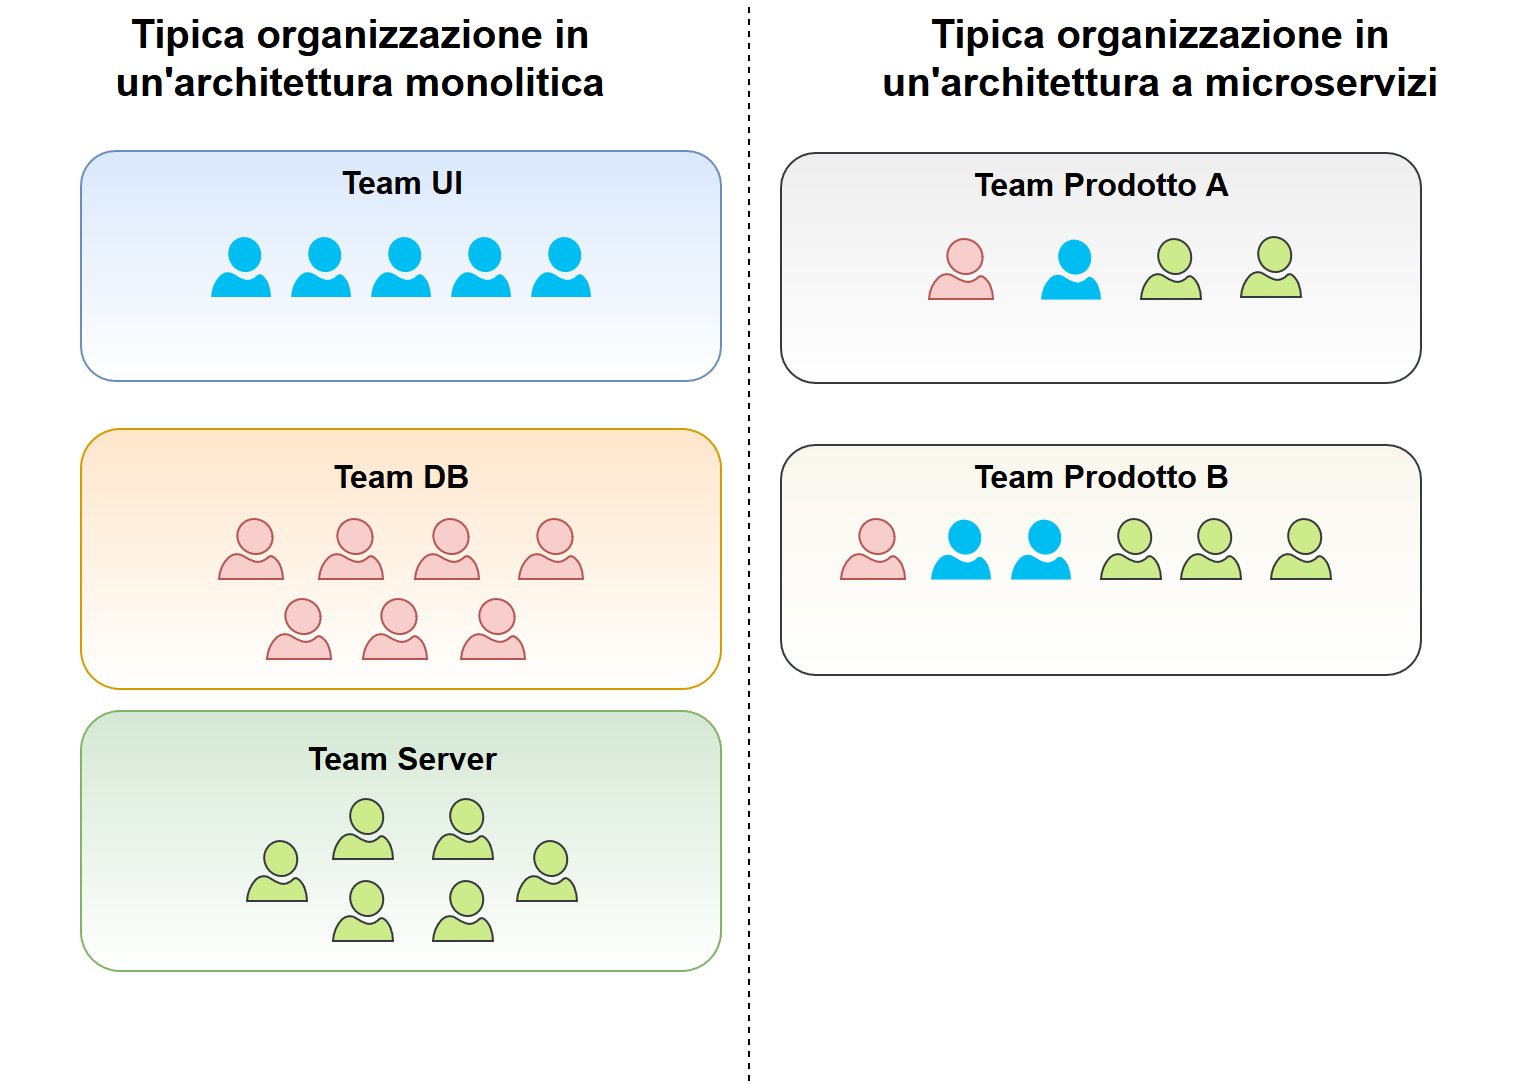
\includegraphics[width=0.9\columnwidth]{intro/business-organization}
  \caption{Illustrazione che mostra la differente organizzazione aziendale in un ambiente di sviluppo monolitico e in un ambiente di sviluppo a microservizi.\\ \cite{site:fowler-microservices}}
  \label{fig:business-organization}
\end{figure}

Quando le persone sono così isolate, anche una semplice modifica può richiedere l'intervento di altre persone in \emph{team} diversi.
La maggiore richiesta di pianificazione e organizzazione tra gruppi di sviluppo diversi causa un peggioramento dell'efficienza del processo di sviluppo.

L'approccio orientato ai microservizi con la suddivisione dell'applicazione invece pone l'accento sulle capacità di business: ogni \emph{team} inerente un particolare settore di business si occupa dell'intero prodotto per quel settore (sviluppando interamente UI, DB, ecc.).
I \emph{team} in questo approccio sono multidisciplinari e gli scambi con altri settori riflettono le effettive dipendenze tra un settore e un altro all'interno dell'azienda.
\footcite{site:fowler-microservices}

Un esempio di quest'approccio alla suddivisione lo si ritrova in Amazon, dove vige il motto "you build, you run it" ("tu lo costruisci, tu lo esegui").
In Amazon ogni \emph{team} ha completa responsabilità del prodotto anche in ambiente di produzione, mettendo in comunicazione diretta sviluppatori e utenti del prodotto per le attività di supporto e manutenzione.
\footcite{site:amazon-microservices}

Le comunicazioni tra servizi sono orchestrate usando semplici protocolli basati su REST.
REST, acronimo di REpresentational State Transfer, è un tipo di architettura \emph{software} per lo sviluppo di applicazioni distribuite, introdotta nel 2000 nella tesi di dottorato di Roy Fielding.
Le architetture basate su REST prevedono che la scalabilità delle applicazioni sia conseguenza di pochi principi di progettazione:

\setlist{nolistsep}
\begin{itemize}
  \item separazione tra \emph{client} e \emph{server}: i ruoli delle due componenti sono ben distinti utilizzando un insieme di interfacce comuni per la comunicazione, permettendo quindi uno sviluppo indipendente di queste componenti (se l'interfaccia comune non viene alterata);
  \item \emph{stateless}: la comunicazione \emph{client-server} è vincolata in modo che nessuna informazione sullo stato del \emph{client} venga memorizzata dal \emph{server};
  \item \emph{cacheable}: ogni \emph{client} deve poter memorizzare le risposte inviate dal \emph{server} per minimizzare le comunicazioni \emph{client-server}. Ogni risposta deve comunicare al \emph{client} implicitamente o esplicitamente se essa è memorizzabile;
  \item \emph{layered system}: un \emph{client} non deve poter discernere un \emph{server} di basso livello da uno intermedio, dedicato a migliorare le prestazioni o introdurre politiche di sicurezza;
  \item \emph{uniform interface}: la comunicazione tra \emph{client} e \emph{server} deve avvenire con un'interfaccia omogenea, disaccoppiando le due componenti ma degradando potenzialmente l'efficienza, dal momento che le informazioni vengono trasferite in una forma standardizzata invece di una più affine alla loro struttura.
\end{itemize}
\footcite{site:rest-wiki}
\footcite{rest-thesis}

L'esperienza di Fowler mostra come siano due le tipologie di protocolli più usati nelle architetture a microservizi:
\setlist{nolistsep}
\begin{itemize}
  \item protocolli basati su richieste/risposte HTTP secondo API ben dettagliate;
  \item protocolli basati sullo scambio di messaggi in un canale di comunicazione snello. I servizi producono e consumano i messaggi che circolano nel canale di comunicazione, secondo regole di accesso definite.
\end{itemize}

Quando un'applicazione è suddivisa in molteplici componenti sorgono naturalmente dubbi sulla gestione delle informazioni che ciascuna componente gestisce.
Solitamente nelle architetture monolitiche gli analisti astraggono i domini dell'applicazione scegliendo una fra le tecniche di modellazione disponibili e applicandola a tutti i domini;
i modelli prodotti sono poi veicolati su singoli \emph{storage} di dati (ad es. unico \emph{database}).
L'architettura a microservizi invece propone di concepire i modelli in autonomia per ogni singolo servizio, utilizzando le tecniche ritenute più appropriate.
Questa decentralizzazione dell'astrazione dei modelli si riflette anche sulla possibilità di decentralizzare le decisioni relative a quale \emph{storage} dei dati utilizzare per ciascun servizio.
Nell'architettura a microservizi si preferisce che ogni servizio gestisca il proprio \emph{database} in base ai requisiti che il servizio deve soddisfare: il database di un servizio potrebbe essere un'istanza di una stessa piattaforma tecnologica, una piattaforma specifica e ottimizzata per il caso d'uso del servizio oppure potrebbe non essere utilizzato (servizi puramente funzionali).
Questo approccio alla gestione della persistenza è chiamato \emph{Polyglot Persistence} ed è utilizzabile anche in architetture monolitiche, malgrado appaia con maggior frequenza in architetture a microservizi.
\footcite{site:fowler-microservices}

\begin{figure}[H]
    \centering
    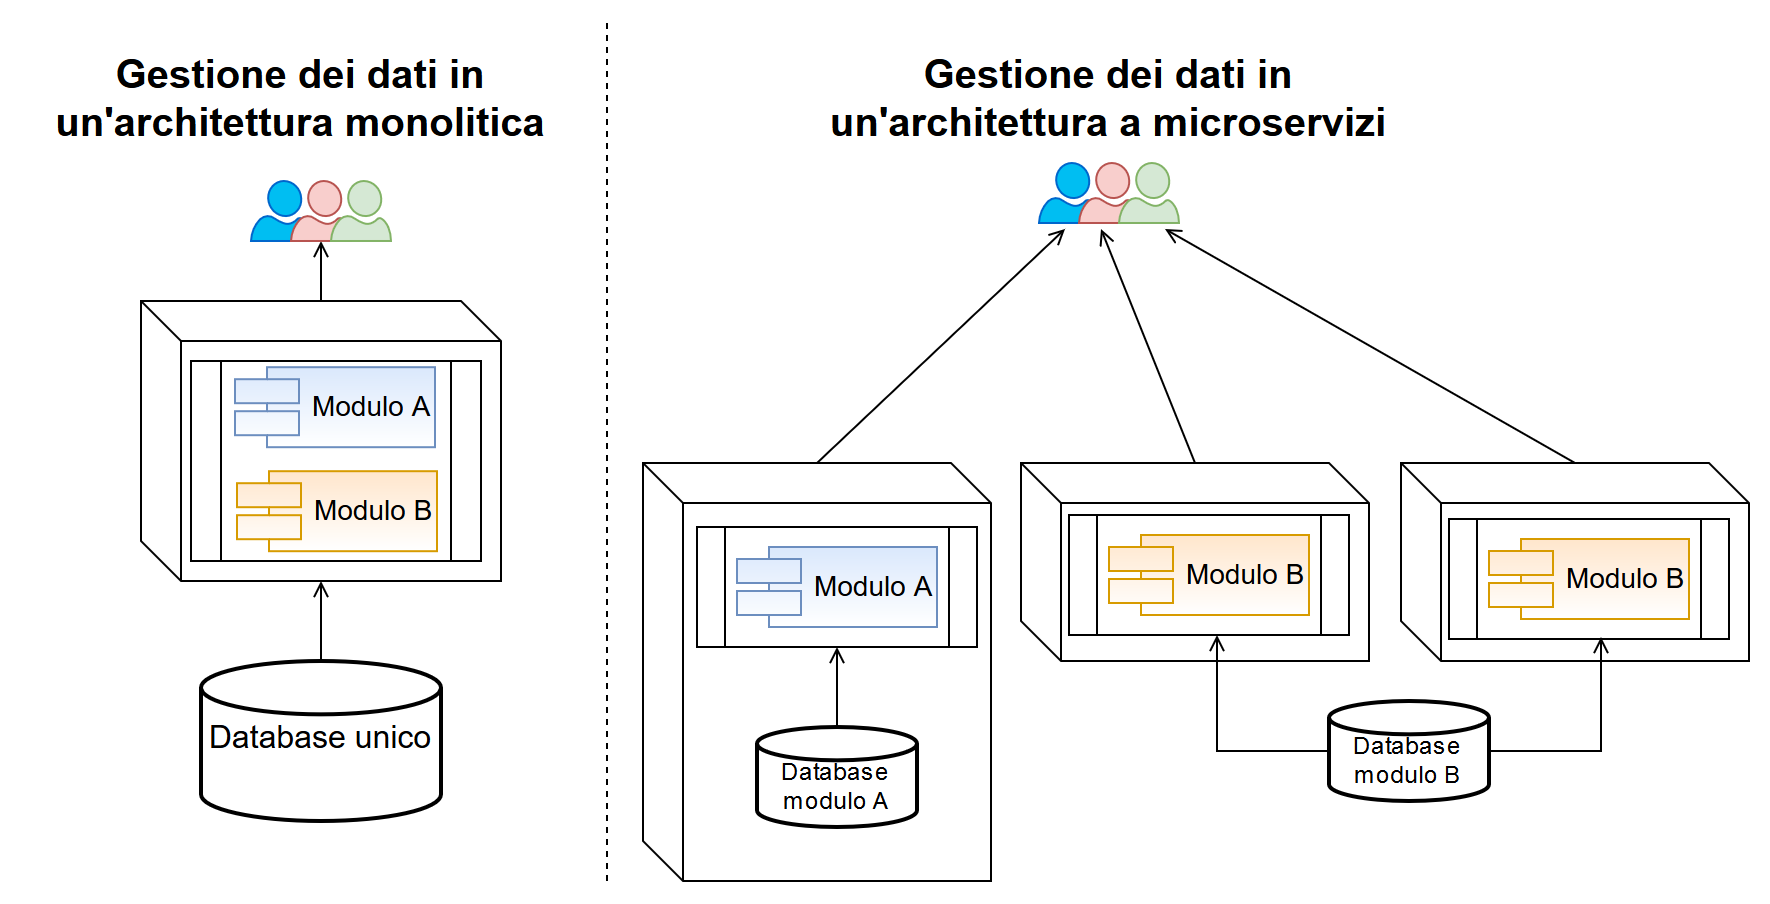
\includegraphics[width=0.9\columnwidth]{intro/data-storage}
    \caption{Illustrazione che mostra la differente gestione dell'architettura di persistenza dei dati tra prodotti software con architettura monolitica e con architettura a microservizi.\\ \cite{site:fowler-microservices}}
    \label{fig:data-storage}
\end{figure}

Le decisioni di \emph{storage} decentralizzate implicano una maggior attenzione verso gli aggiornamenti dei dati.
Fowler rileva che l'approccio comune agli aggiornamenti in un'architettura monolitica è quello di usare le transazioni per garantire la consistenza dei dati prima e dopo ciascun aggiornamento.
L'utilizzo di transazioni è un grave limite per l'architettura a microservizi, in quanto le transazioni impongono un ordine temporale che potrebbe non essere rispettato, causando inconsistenze dei dati salvati.
É per questo che le architetture a microservizi enfatizzano l'utilizzo di comunicazioni non vincolanti (\emph{transactionless}): eventuali inconsistenze vengono segnalate e risolte grazie a operazioni correttive.
\footcite{site:fowler-microservices}

Una conseguenza nell'utilizzo dei servizi come componenti è che le applicazioni devono prevedere e tollerare malfunzionamenti nei servizi. L'utilizzatore dei servizi deve quindi rispondere ai malfunzionamenti nel modo più elegante possibile.
É naturale quindi attribuire l'aumento di complessità della gestione dei malfunzionamenti tra i difetti delle architetture a microservizi.
Dal momento che i servizi possono malfungere in ogni momento, è fondamentale riuscire a:

\setlist{nolistsep}
\begin{itemize}
  \item monitorare il servizio,
  \item segnalare il malfunzionamento e
  \item ripristinare automaticamente il servizio
\end{itemize}
nel più breve tempo possibile. Conseguentemente, ogni servizio deve essere progettato focalizzando l'attenzione sulle attività di monitoring, individuando le metriche rilevanti (ad es. \emph{throughput}, latenza, ecc.).

Uno dei temi cruciali che ho riscontrato nella trattazione di Fowler consiste nel chiedersi quante responsabilità debba avere ciascun servizio: secondo Fowler la caratteristica fondamentale da osservare è la nozione di sostituzione e aggiornamento indipendenti.
Un buon segnale lo si ritrova quando ad ogni modifica di un servizio, questa modifica non richiede adattamenti in altri servizi (a meno di modifiche alle funzionalità offerte).
Se due o più servizi vengono aggiornati spesso insieme probabilmente essi dovrebbero essere uniti.
\footcite{site:fowler-microservices}

%**************************************************************
\pagebreak
\section{Valutazione dei rischi considerati nello stage}

\subsection{Valutazione dei rischi di uno stage interno}

Lo stage formativo viene previsto dal CdL triennale di Informatica in due modalità:
\setlist{nolistsep}
\begin{itemize}
  \item stage aziendali, riferiti anche come stage esterni, per i quali il proponente del progetto di stage è un'azienda;
  \item stage non aziendali, riferiti anche come stage interni individuali, per i quali il proponente del progetto di stage è un docente dell'Ateneo di Padova.
\end{itemize}


Sebbene lo stage aziendale sia la modalità preferita per svolgere l'attività, mi sono imbattuto in due ostacoli che mi hanno portato ad avviare uno stage interno. \\
Il mio stato di studente lavoratore causa il primo ostacolo: l'azienda per cui sono assunto non poteva offrire stage riguardanti il settore IoT.
Nel momento in cui ho iniziato a cercare proposte di stage e mi sono quindi informato sulle modalità con cui avrei potuto assentarmi da lavoro,
l'ufficio per le risorse umane dell'azienda per cui sono assunto mi ha comunicato che avrei avuto opzioni limitate, dipendenti dal motivo dell'assenza. \\
Se l'assenza avesse comportato l'inizio di attività lavorative per altre aziende (concorrenti oppure non concorrenti) sarei stato costretto a scegliere tra due opzioni:
\setlist{nolistsep}
\begin{itemize}
  \item il licenziamento dall'azienda per cui sono assunto;
  \item l'avvio della procedura di \gls{aspettativag} del lavoro come prevista dalla legge 53 recante data 8 marzo 2000. \footcite{site:aspettativa}.
\end{itemize}
Quindi fin dall'inizio la ricerca di un progetto di stage aziendale è stata fortemente messa in discussione dalle menzionate opzioni. \\
Malgrado il primo ostacolo, ho proseguito la ricerca dello stage aziendale al fine di ponderare se gli aspetti negativi legati al congedo lavorativo potessero essere in qualche modo bilanciati da eventuali esperienze formative.
\\
Dato il periodo di inizio dello stage (ottobre/novembre 2017), molti degli stage aziendali riguardanti il settore IoT proposti erano già stati svolti da altri studenti del corso.
Le poche proposte di stage aziendale legate al settore IoT rimanenti erano interessate alla integrazione con prodotti già esistenti:
malgrado l'opportunità offerta da queste aziende fosse interessante, ho riflettuto a lungo sul fatto che l'attività formativa non fosse adeguatamente supportata. \\
Nei progetti proposti infatti le aziende proponenti hanno enfatizzato l'utilizzo degli strumenti interni da loro sviluppati, da una parte per motivarmi ad essere assunto al termine dello stage,
dall'altra per effettivamente semplificarmi il lavoro nel processo di sviluppo. \\ \\
L'aspetto formativo è stato l'ambito più discusso per effettuare la scelta: malgrado la presenza di esperti nel settore mi interessasse,
per l'opportunità di approfondire l'ambito d'uso reale dei dispositivi \emph{smart}, la scelta di legarmi a un singolo prodotto, non particolarmente diffuso e utilizzato,
mi ha spinto ad iniziare a valutare il percorso di stage interno. \\

Ho riassunto i rischi considerati per lo svolgimento di uno stage interno individuale nella tabella ~\ref{tab:rischi-stage-interno}.

\begin{table}
\caption{Tabella di analisi dei rischi correlati allo svolgimento di uno stage interno}
\label{tab:rischi-stage-interno}
\begin{tabularx}{\linewidth}{|p{7.5cm}|X|X|}
\hline
\textbf{Rischio} & \textbf{Probabilità di accadimento} & \textbf{Gravità del danno potenziale}\\
\hline
Il lavoro svolto individualmente, senza possibilità di essere guidato da esperti nel settore, potrebbe risultare ininfluente. La presenza di una persona con più esperienza in un determinato tema è utile in quanto può focalizzare l'attenzione su problematiche reali, le quali potrebbero non essere correttamente valutate nel momento in cui si dispone di scarsa esperienza in materia. & Molto probabile & Grave \\
\hline
Il lavoro svolto individualmente, senza possibilità di essere guidato da esperti nel settore, potrebbe procedere più lentamente, causando il non raggiungimento degli obiettivi preposti. & Molto probabile & Media \\
\hline
\end{tabularx}
\end{table}


\subsection{Valutazione dei rischi del tema IoT}

Nuove tecnologie contengono sempre una determinata quantità di rischi: mentre la maggior parte degli sviluppatori trovano utilizzi per i dispositivi IoT,
altri cercano modi per usarli per scopi meno nobili. \\
I dispositivi IoT stanno sempre più diffondendosi in molti aspetti su cui basiamo la società moderna:
\setlist{nolistsep}
\begin{itemize}
  \item trasporti;
  \item comunicazione;
  \item settore energetico.
\end{itemize}

Attacchi informatici contro questi dispositivi possono portare al caos: dalla distruzione di proprietà alla messa in discussione della propria sicurezza, con l'accezione che il termine \emph{safety} possiede nella lingua inglese.
A peggiorare la situazione, gli acquirenti di questi dispositivi pretendono che essi continuino a funzionare per una quantità di tempo superiore a quella che il consumismo tecnologico ha abituato. \\
La quantità di protocolli sviluppati per l'IoT porta ad aumentare la complessità insita in questi dispositivi.
Una complessità maggiore implica un maggior costo per le società per aggiornare i prodotti rilasciati, portando quindi i produttori ad abbandonare i dispositivi rilasciati da più tempo, ignorando l'insorgere di nuove vulnerabilità.

Date le suddette premesse, per il settore IoT ho posto numerose osservazioni relative ai rischi collegati allo sviluppo di prodotti software e hardware. I rischi considerati sono riassunti nella tabella ~\ref{tab:rischi-iot}.
\begin{table}[H]
\caption{Tabella di analisi dei rischi correlati al tema IoT}
\label{tab:rischi-iot}
\begin{tabularx}{\linewidth}{|p{7.5cm}|X|X|}
\hline
\textbf{Rischio} & \textbf{Probabilità di accadimento} & \textbf{Gravità del danno potenziale}\\
\hline
Lo sviluppo di prodotti legati all'IoT espone l'utente degli stessi a possibili rischi di cybersicurezza: il furto di dati ma soprattutto la perdita di controllo dell'utente sui propri dispositivi sono scenari possibili e con conseguenze disastrose per lo sviluppatore di tale prodotto. & Probabile & Molto grave \\
\hline
La mole di dati raccolta dai dispositivi inseriti in un contesto IoT potrebbe essere tale da richiedere investimenti consistenti per la loro elaborazione e per mantenere elevata la loro confidenzialità. Inoltre la diversità dei dispositivi presenti in una rete aumenta la complessità del trattamento delle informazioni. & Probabile & Media \\
\hline
Dal momento che l'IoT è un ambito emergente nel contesto ITC ho osservato la nascita di una multitudine di protocolli per la raccolta e la trasmissione delle informazioni, nessuno dei quali è stato indicato o si è imposto come standard globale. & Molto probabile & Media \\
\hline
\end{tabularx}
\end{table}


\subsection{Valutazione dei rischi dell'architettura a microservizi}

L'architettura a microservizi permette di sviluppare un'applicazione complessa partendo da piccole e relativamente isolate componenti;
in questo modo i cambiamenti effettuati sono facilmente verificabili.
La frammentazione dell'architettura del prodotto rende tuttavia più complesse le attività di test funzionali, perché per eseguire un tipico caso d'uso di una funzionalità completa sono richiesti molteplici servizi, correttamente configurati per comunicare tra loro ed eseguire simultaneamente. \\ \\
Lo sviluppo di servizi indipendenti rende inoltre difficoltosa l'attività di integrazione delle modifiche: nel momento in cui molti \emph{team} di sviluppo lavorano ciascuno nel proprio servizio non è possibile integrare queste modifiche senza una attenta pianificazione, che coinvolga la comunicazione dei cambiamenti effettuati. \\
Nel mio caso questo non si applica, lavorando individualmente, tuttavia mi sono comunque richieste le attività di allineamento delle funzionalità tra i servizi che necessitano di comunicare tra loro. \\ \\
Anche in questo caso, la relativa novità dell'argomento causa una generale mancanza di documentazione pratica, lasciando lo spazio ad esempi semplici, che non riflettono applicazioni d'uso reale, oppure documentazione teorica, che non si spinge ad analizzare problematiche reali.
La tabella ~\ref{tab:rischi-arch-microservizi} riassume e sintetizza i rischi analizzati in precedenza.

\begin{table}[H]
\caption{Tabella di analisi dei rischi correlati all'utilizzo dell'architettura a microservizi}
\label{tab:rischi-arch-microservizi}
\begin{tabularx}{\linewidth}{|p{7.5cm}|X|X|}
\hline
\textbf{Rischio} & \textbf{Probabilità di accadimento} & \textbf{Gravità del danno potenziale}\\
\hline
Spostamento di alcune problematiche di progettazione da un livello di modulo a un livello di architettura del sistema. & Probabile & Media \\
\hline
Le performance dell'applicazione sviluppata potrebbero non essere sufficienti passando da un'architettura monolitica a una a microservizi. & Scarsamente probabile & Grave \\
\hline
Difficoltà nel reperimento delle informazioni, data la relativa novità dell'argomento. Assume maggior significato nel momento in cui l'esperienza con un tale paradigma risulti scarsa o nulla. & Molto probabile & Grave \\
\hline
\end{tabularx}
\end{table}

\section{Organizzazione dello Stage}

Ho pianificato le attività, in termini di quantità di ore di lavoro, secondo la tabella ~\ref{tab:organizzazione-stage} e le ho inserite in un Piano di Lavoro.
Dal momento che ho già avuto modo di trattare il lato tecnologico del progetto nel corso del percorso di studi, ho allocato 40 ore di formazione negli argomenti meno conosciuti e li ho suddivisi in due parti:
\begin{itemize}
  \item una prima parte in cui ho studiato le caratteristiche comuni delle architetture a microservizi e i Design Pattern nati per facilitare l'implementazione di un sistema con questo tipo di architettura;
  \item una seconda parte pratica di applicazione dei princìpi teorici in Node.js e il ripasso della caratteristiche tecniche del \emph{framework} React.
\end{itemize}
Durante quest'insieme di attività di formazione, per mitigare i rischi elencati in tabella ~\ref{tab:rischi-stage-interno}, ho focalizzato la mia attività di studio alla ricerca di esempi sviluppati da aziende con esperienza in materia per risolvere i problemi che hanno dovuto affrontare.
Il secondo macroblocco di attività riguarda l'analisi, la progettazione e l'implementazione dei servizi di comunicazione con i dispositivi. A queste attività ho allocato 120 ore, in quanto per mitigare le probabilità di incorrere nei rischi elencati in tabella ~\ref{tab:rischi-iot} ho assegnato risorse per l'attività di ricerca del protocollo di comunicazione da implementare. Durante le attività di analisi inoltre mi sono preparato per contrastare i rischi più probabili che ho menzionato in tabella ~\ref{tab:rischi-arch-microservizi}, analizzando i requisiti funzionali del sistema e mettendoli in relazione con le attività di ricerca effettuate durante le attività di formazione. Ho incluso nelle attività di progettazione di questo blocco anche la progettazione e realizzazione dei dispositivi "virtualizzati", l'implementazione dei quali mi ha permesso di effettuare i primi test dei servizi di comunicazione.
Il terzo macroblocco di attività riguarda l'analisi dell'interazione che un \emph{client} può avere con i servizi di comunicazione, permettendomi di arrivare alla progettazione e realizzazione del servizio che compone le funzionalità da offrire alla \emph{dashboard} e la \emph{dashboard} stessa.
L'ultimo blocco di attività riguarda la revisione del prototipo implementato e la sua possibile pubblicazione sulla piattaforma di Heroku\footcite{heroku}.

\begin{table}[H]
	\caption{Tabella che illustra la pianificazione delle attività dello stage}
	\label{tab:organizzazione-stage}
	\begin{tabular}{|>{\centering} m{1.5cm}|>{\centering} m{1.5cm}|m{10cm}|}
		\hline
		\multicolumn{2}{|c|}{\textbf{Durata in ore}} & \textbf{Descrizione dell'attività} \\
		\hline
		\multicolumn{2}{|c|}{40} & Formazione
	 	\begin{itemize}
			\item Architettura microservizi
			\item Node.JS orientato ai microservizi
			\item React
		\end{itemize}
		\\
		\hline
		\multirow{4}{*}{120} & & Analisi, sviluppo e implementazione servizi di comunicazione con i dispositivi IoT\\
		\cline{2-2}
		& 40 & \begin{itemize}
			\item Analisi dei protocolli \emph{open source} esistenti per i diversi dispositivi IoT
			\item Stima implementazione eventuali nuovi protocolli
			\end{itemize} \\
			\cline{2-2}
			& 80 & \begin{itemize}
			\item Progettazione dei servizi di comunicazione con i dispositivi
			\item Progettazione dei test dei servizi di comunicazione
			\item Realizzazione dei test e dei servizi di comunicazione in Node.js
		\end{itemize} \\
		\hline
		\multirow{4}{*}{120} & & Analisi, sviluppo e implementazione servizio di presentazione delle informazioni agli utenti\\
		\cline{2-2}
		& 40 & \begin{itemize}
		\item Analisi interazione utente con la \textit{dashboard}
		\end{itemize} \\
		\cline{2-2}
		& 80 & \begin{itemize}
			\item Progettazione del servizio di presentazione informazioni
			\item Progettazione dei test del servizio di presentazione
			\item Realizzazione dei test e del servizio di presentazione in React, HTML5 e CSS3.
		\end{itemize} \\
		\hline
		\multicolumn{2}{|c|}{20} & {\textit{Review} dei servizi, \textit{deploy} dei servizi su Heroku.}\\
		\hline
		\multicolumn{2}{|c|}{\textbf{Totale ore}} & {\textbf{300}} \\
		\hline
\end{tabular}
\end{table}
% Le settimane sono composte da 40 ore totali di impegno sul progetto,

\section{\emph{Milestone}}
In questa sezione presento le \gls{milestone} previste per il progetto su base settimanale, associando a ciascuna \emph{milestone} i prodotti che devono essere sviluppati entro la corrispondente scadenza.
\begin{itemize}
	\item Prima settimana: Completamento delle attività di autoformazione con produzione di una breve relazione riguardante la stessa;
	\item Seconda e terza settimana: Analisi dei protocolli di comunicazione esistenti, primo ciclo di progettazione e implementazione del servizio di comunicazione, mirato all'implementazione dei dispositivi \textit{virtualizzati};
	\item Quarta e quinta settimana: Revisione analisi sui protocolli, secondo ciclo di progettazione e implementazione del servizio di comunicazione, mirato all'implementazione dei dispositivi fisici (Raspberry Pi);
	\item Sesta e settima settimana: Analisi dell'interazione utente con la \emph{dashboard}, progettazione e implementazione del servizio di presentazione;
	\item Ottava settimana: Revisione dei servizi, stesura del Manuale d'Uso e deploy (opzionale) di un ambiente di simulazione della \emph{dashboard} su Heroku.
\end{itemize}
